\documentclass{article}
\usepackage{graphicx}
\usepackage{hyperref}
\usepackage{float}
\usepackage{caption}
\usepackage{pdfpages}

\title
{
	Practica 6 y 7\\
	Algoritmos de Grafos
}

\author
{
	Adolfo Roman Jimenez
}

\begin{document}
	
	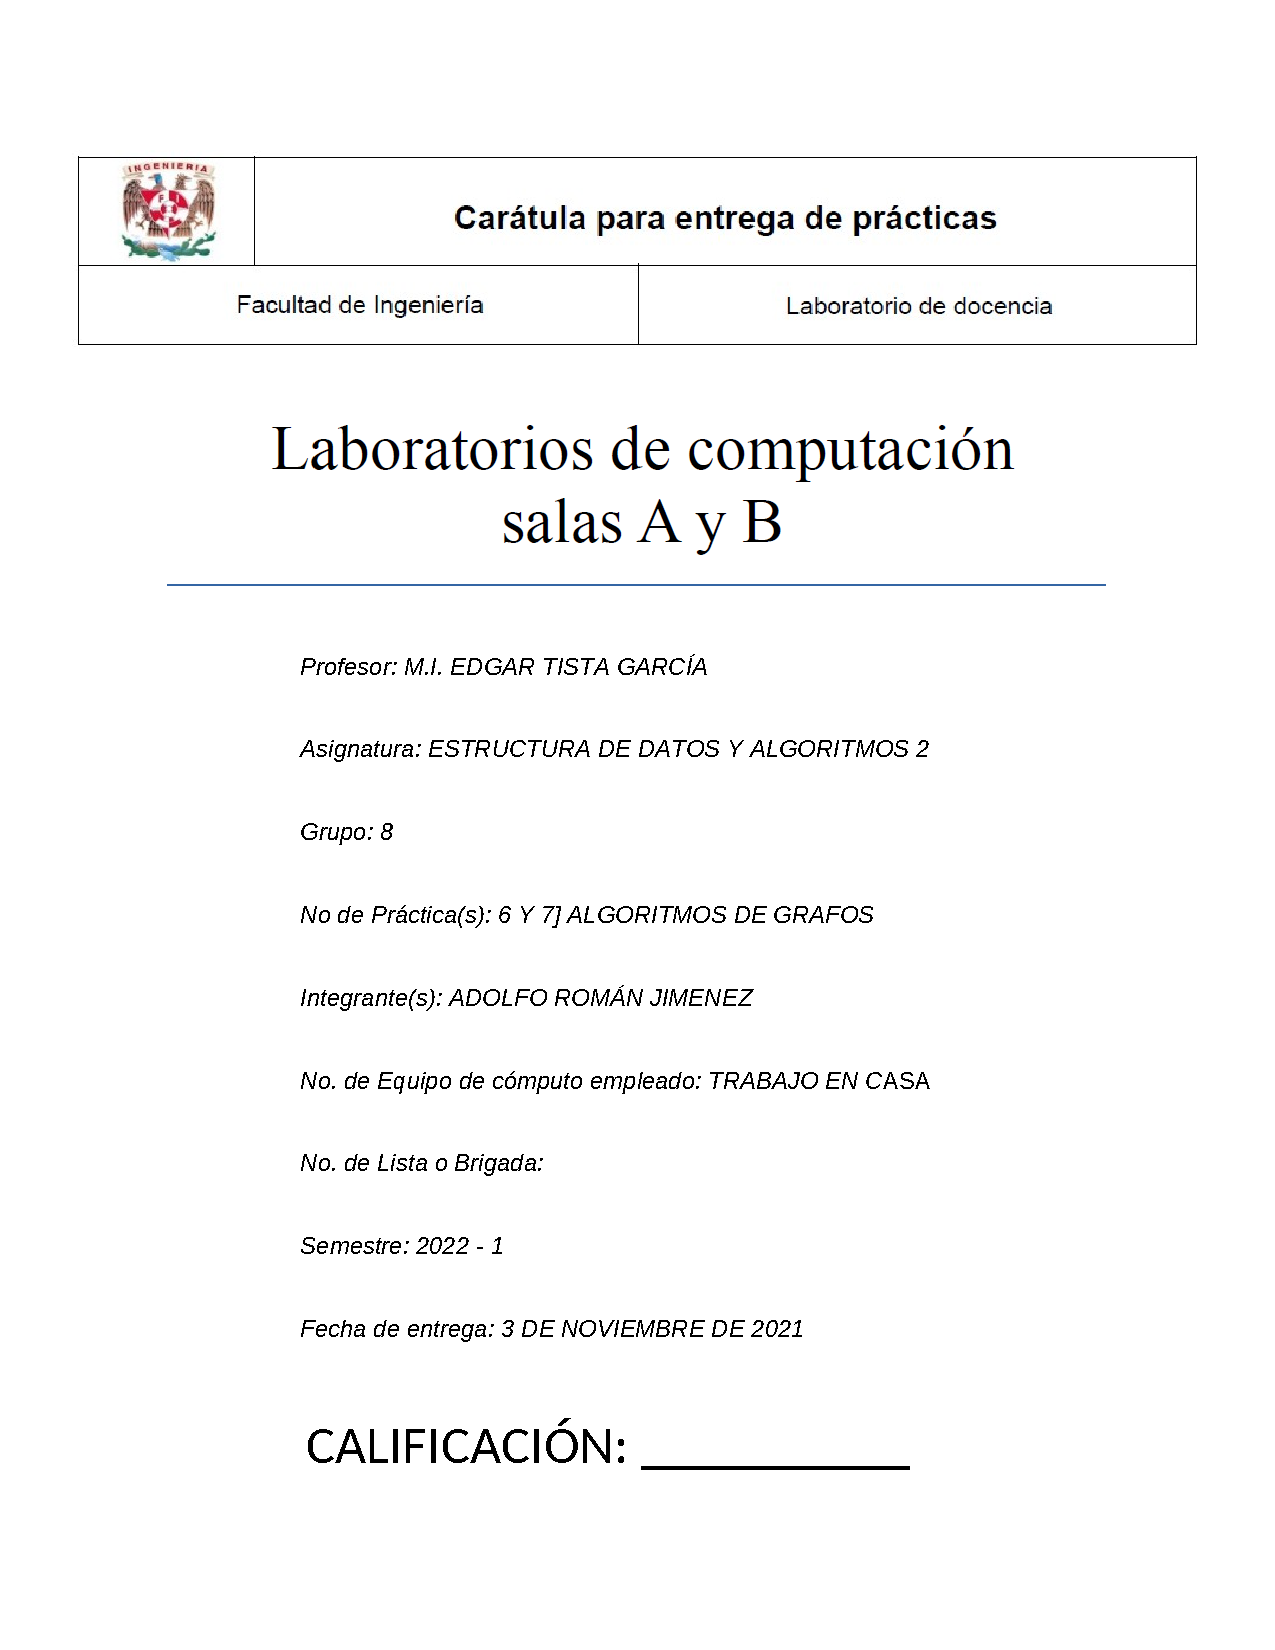
\includepdf{c6y7.pdf}
	
	\maketitle
	
	\section{Objetivo General}
	
	El estudiante conocerá las formas de representar un grafo e identificará las
	características necesarias para comprender el algoritmo de búsqueda por expansión y	profundidad.
	
	\section{Objetivo de Clase}
	
	El alumno será capaz de implementar y comprender los grafos, así como los
	recorridos. 
	
	\newpage
	
	\section{Actividades}
	
		\subsection{Ejercicio 1.1}
		
			\subsubsection{Desarrollo}
			
			
				La clase \emph{Graph} primeramete comienza importando a \emph{LinkedList} para poder usarla dentro del programa.\\
				
				Ya dentro de la clase, el programa primero declara una variable entera \textbf{V} y una referencia a una lista de listas de enteros llamada \textbf{adjArray}.\\
				
				Para el constructor de la clase llamado \emph{Graph()} este constructor usa como parametro una variable entera \textbf{v} y ya dentro del constructor, primeramente se iguala la variable \textbf{v} a la variable \textbf{V} y se crea el objeto de listas ligadas que se asocia a la referencia en \textbf{adjArray}, despues de esto, por medio de un \textit{for-loop} que itera hasta \textbf{v} se insertan dentro de cada uno de los indices en \textbf{adjArray} un numero \textbf{v} de listas ligadas que contendran a numeros enteros.\\
				
				Despues de esto, la clase contiene tambien al metodo \emph{addEdge()} el cual usa de parametros a las variables enteras \textbf{v} y \textbf{w} y lo que este metodo hace, es que toma, dentro de \textbf{adjArray}, primeramente el indice de la lista en \textbf{v} y agrega el entero \textbf{w}, despues de forma inversa, toma el indice de la lista en \textbf{w} y agrega el entero \textbf{v}.\\
				
				Por ultimo el metodo \emph{printGraph()} es un \textit{for-loop} que itera desde 0 hasta \textbf{V} y que imprime la leyenda \textbf{"Lista de adyacencia del vertice \textit{x}"} siendo \textbf{x} el nodo a imprimir.\\
				
				Despues de esto el programa vuelve a imprime el numero del nodo y con un \textit{enhanced loop} que imprime los enteros dentro del nodo \textbf{v} imprime en pantalla cada uno de los elementos que el nodo contenga.\\
				
				Para la clase \emph{Main} en \emph{main()} primeramente se declara una variable entera \textbf{V} que se iguala a 5 y acto seguido se crea una variable de la clase \emph{Graph} llamada \textbf{graph} cuyo constructor contiene como parametro el valor en \textbf{V}.\\
				
				Acto seguido, a traves del metodo \emph{graph.addEdge()} la clase \emph{Main} agrega cada uno de los elementos en cada nodo generado, desde 0 a 4.\\
				
				Por ultimo se imprime la lista del grafo por medio del metodo \emph{graph.printGraph()}\\
				
				La grafica resultante tendria que ser la siguiente:
				
				\begin{figure}[H]
					\centering
					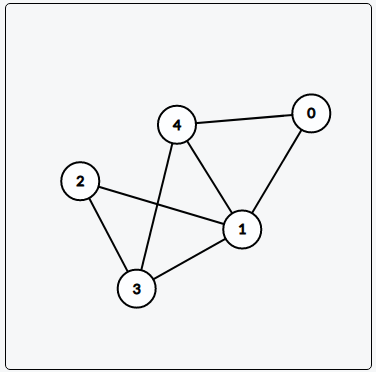
\includegraphics[scale=0.65]{images/graphMain.png}
					\caption*{Ejercicio 1.1: Grafica resultante}
				\end{figure}
							
			\subsubsection{Ejecucion}
				\begin{figure}[H]
					\centering
					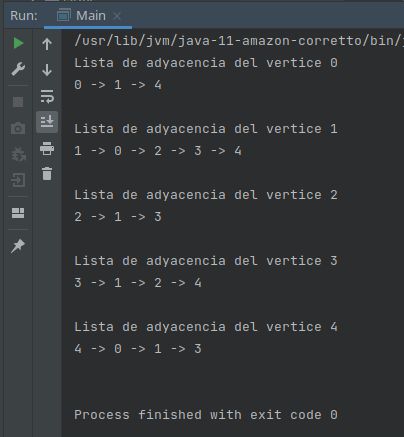
\includegraphics[scale=0.8]{images/e1.png}
					\caption*{Ejercicio 1: Ejecucion de Ejercicio 1}
				\end{figure}
		\newpage
		
		\subsection{Ejercicio 1.2}
		
			\subsubsection{Desarrollo}
			
				Para este ejercicio se creo un menu en la clase principal \emph{Main} y 3 submenus para cada una de las opciones. Esto fue debido a que las diferentes opciones del menu principal necesitan usar metodos especificos que no se pueden aglutinar en un solo menu de opciones.\\
				
				El menu principal contenido en el metodo \emph{menu1()} contiene las siguientes opciones:
				
				\begin{enumerate}
					\item Grafo No Dirigido
					\item Grafo Dirigido
					\item Grafo Ponderado No Dirigido
					\item Grafo Ponderado Dirigido
					\item Salir
				\end{enumerate}
			
				Para la opcion 1 que es la de \textit{Grafo No Dirigido} a traves de un control \textit{Switch()} accede al metodo \emph{option1()}.\\
				
				Inmediatamente despues de que el usuario accede a este metodo, el mismo crea una instancia de la clase \emph{Graph} la cual lleva el nombre de \textbf{uGraph}. Al momento de crear la instancia, el constructor de la clase \emph{Graph} le pregunta al usuario, cuantos nodos desea crear para el grafo. El usuario ingresa el numero de nodos que se depositan en la variable privada \textbf{V} de la clase \emph{Graph} y acto seguido el constructor asigna una \textit{LinkedList<>} a la variable \textbf{nodes} la cual es una lista ligada de instancias de la clase \emph{Node}.\\
				
				Despues de esto, por medio de un \textit{for-loop} se itera hasta el numero de nodos que el usuario desea crear, creando instancias de la clae \emph{Node} que dentro de su estructura incluyen el numero de nodo creado dependiendo de el iterador en ese momento y por medio del metodo \emph{add()} los inserta a la lista \textbf{nodes}.\\   
				
				Despues de esto,a traves de una variable entera \textbf{option1} se asigna una opcion por medio del metodo \emph{menu2}, el cual devuelve un entero dependiendo de la opcion que el usuario escoja.\\
				
				El metodo \emph{menu2()} contiene las siguientes opciones:
				
				\begin{enumerate}
					\item Agregar Conexiones
					\item Imprimir Lista de Adyacencia
					\item Imprimir BFS
					\item Imprimir DFS
					\item Salir
				\end{enumerate}
			
				El metodo \emph{option1()} de igual forma, usa una funcion \textit{switch()} para llevar a cabo la opcion que el usuario haya escogido dentro del submenu. Para la opcion numero 1 que es la de \textit{Agregar conexiones} este \textit{switch()} invoca al metodo \emph{setEdges()} y le asigna dos parametros que son dos variables \textit{string}, \textbf{"u"} y \textbf{"r"} las cuales sirven para indicar que las conexiones a ingresar corresponden a un grafo no dirigido \textbf{"u"} por \textit{undirected} y que es un grafo no ponderado, \textbf{"r"} para \textit{regular}.\\
				
				Dentro del metodo \emph{setEdges()} primero evaluamos que el grafo tenga mas de 1 nodo, de no ser asi, entonces termina el metodo puesto que no existen conexiones para realizar. Si esto es falso, entonces el metodo procede a declarar las variables enteras \textbf{v}, \textbf{w}, \textbf{edges}, \textbf{e}, \textbf{maxedges} y la variable \textit{boolean} \textbf{flag}.\\
				
				Acto seguido se procede a un \textit{swtich()} para determinar, dependiendo del tipo de grafo a crear, el numero maximo de conexiones entre nodos que el usuario puede crear. Para el caso de un grafo no dirigido se iguala entonces la variable \textbf{maxedges} al resultado de la ecuacion $V*(V-1)/2$ donde \textbf{V} es el numero de nodos que el grafo contiene.\\
				
				Una vez terminado esto, se le solicita al usuario el numero total de conexiones que desea crear y dentro de un \textit{while-loop} se verifica que el usuario ingrese un numero que no sea mayor al total maximo de conexiones posibles para el nodo, valor que esta contenido en \textbf{maxedges}.\\
				
				Una vez verificado esto, el programa permite al usuario ingresar las conexiones entre nodos que desee agregar, el metodo verifica que el usuario agregue conexiones entre nodos que existan y que no agregue un nodo que sea mayor a la cantidad de nodos existentes.\\
				
				Este metodo de igual forma verifica que el nodo no contenga ya la conexion que el usuario desea insertar, si esta conexion ya existe dentro del nodo, el programa le pide al usuario ingresar un valor diferente y le menciona que esa conexion ya se encuentra en el nodo.\\
				
				Por ultimo el metodo verifica tambien que el nodo en el que desea ingresar el usuario la conexion no este ya lleno, esto quiere decir que ya se encuentre totalemente conectado a todos los nodos posibles dentro de su campo, si esto sucede, el programa le menciona al usuario que el nodo ya esta lleno.\\
				
				Si no ha habido ningun problema en este aspecto, entonces se procede a un nuevo \textit{switch()} que verifica cual es el tipo de grafo con el que se esta trabajando. Para este caso como tenemos un grafo no dirigido y no ponderado, el \textit{switch()} invoca al metodo \emph{uGraphNodeAdd()}.\\
				
				Este metodo contiene los parametros enteros \textbf{v} y \textbf{w} que incluyen los nodos que el usuario pretende conectar. Lo que hace el metodo es que simplemente invoca dos veces al metodo \emph{dGraphNodeAdd()} con los parametros invertidos. El metodo \emph{dGraphNodeAdd()} obtiene de la lista \textbf{nodes.next} el indice \textbf{v} y dentro de este agrega la referencia al nodo \textbf{w} a su lista ligada. De igual manera lo hace pero ahora de forma invertida despues cuando ahora obtiene el nodo que esta en la lista \textbf{nodes.next} en el indice \textbf{w} y agrega la referencia al nodo \textbf{v} dentro de esa lista.\\
				
				De esta forma ambos nodos quedan interconectados pues tanto uno como otro contienen su propia informacion.\\
				
				Al finalizar, el usuario puede escoger la opcion 2 \textit{Imprimir Lista de Adyacencia} para corroborar el funcionamiento del programa.
				
							
			\subsubsection{Ejecucion}
			
			\begin{figure}[H]
				\centering
				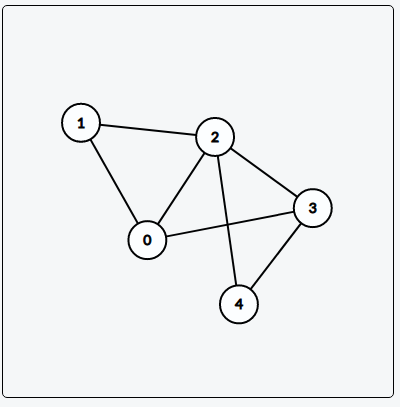
\includegraphics[scale= 0.6]{images/e12graph.png}
				\caption*{Ejercicio 1.2: Grafo a representar}
			\end{figure}
		
			\begin{figure}[H]
				\centering
				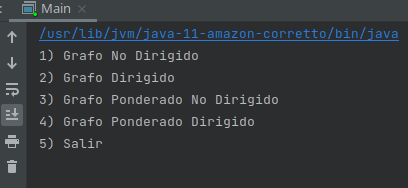
\includegraphics[scale= 0.9]{images/e121.png}
				\caption*{Ejercicio 1.2: Menu Principal}
			\end{figure}
	
			\begin{figure}[H]
				\centering
				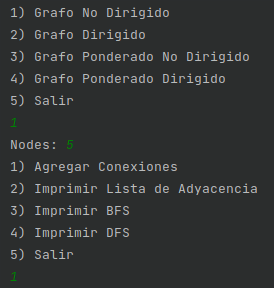
\includegraphics[scale= 0.9]{images/e122.png}
				\caption*{Ejercicio 1.2: submenu2, se agregan nodos}
			\end{figure}
		
			\begin{figure}[H]
				\centering
				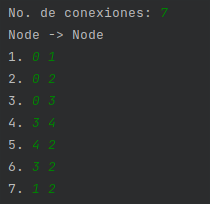
\includegraphics[scale= 1]{images/e123.png}
				\caption*{Ejercicio 1.2: Opcion 1, se agregan conexiones}
			\end{figure}
		
			\begin{figure}[H]
				\centering
				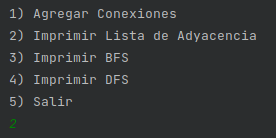
\includegraphics[scale= 1]{images/e124.png}
				\caption*{Ejercicio 1.2: Se imprimen la lista de adyacencia}
			\end{figure}
		
			\begin{figure}[H]
				\centering
				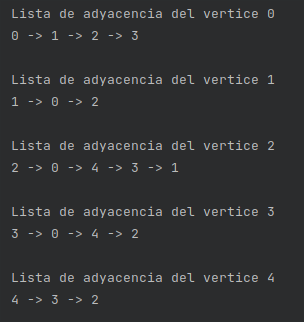
\includegraphics[scale= 1]{images/e125.png}
				\caption*{Ejercicio 1.2: Se visualiza la lista}
			\end{figure}
		
		\newpage
			
		\subsection{Ejercicio 2}
		
			\subsubsection{Desarrollo}
			
				Para este ejercicio como ya se ha descrito anteriormente, se modifico el metodo \emph{setEdges()} para que en este caso generara grafos dirigidos.\\
				
				Se sigue la misma logica del ejercicio anterior, pero en este caso ahora, en el menu principal, el usuario debe seleccionar la opcion 2 que corresponde a \textit{Grafo Dirigido}.\\
				
				Al seleccionar esta opcion, el usuario invoca al metodo \emph{option2()} cuyo menu contiene exactamente las mismas opciones que el ejercicio anterior, de igual manera se crea un grafo al tiempo que el usuario ingresa al metodo \emph{option2()} pero en este caso, el grafo que el programa crea lleva el nombre de \textbf{dGraph}.\\
				
				La diferencia principal es que al momento de escoger en el \emph{menu2()} la opcion de \textit{Crear Conexiones}, ahora el \textit{switch()} de \emph{option2()} invocara al metodo \emph{setEdges()} pero con los parametros \textbf{"d"} y \textbf{"r"} que corresponden a \textit{"directed"} y \textit{"regular"}.\\
				
				Ya dentro de el metodo \emph{setEdges()} el funcionamiento es similar, pero al momento de otorgar un valor a la variable \textbf{maxedges} el programa evalua $V*(V - 1)$ unicamente, puesto que son el total de conexiones que puede obtener un grafo no dirigido.\\
				
				Ya despues de solicitar los nodos a conectar y haberlos ingresado, el programa dentro del \textit{switch()} de \emph{setEdges()} de acuerdo con los parametros de la funcion, invoca al metodo \emph{dGraphAddNodes()} que toma a los parametros \textbf{v} y \textbf{w} que contienen los nodos a conectar de (Nodo \textbf{v} a Nodo \textbf{w}) y toma en la lista \textbf{Node.next} el indice de \textbf{v} y le agrega la referencia a su lista ligada interna del nodo \textbf{w}.\\
				
				Esto se ejecuta hasta que se ha terminado de iterar en las conexiones que el usuario desea crear.\\
				
				Para la ejecucion vamos a tomar el mismo grafo anterior, pero ahora lo haremos como grafo dirigido.\\
				
				Al finalizar la ejecucion, podremos apreciar como las listas de adyacencia tanto del primer ejercicio como del segundo, son totalmente distintas. De hecho se aprecia al finalizar la ejecucion en este ejercicio, como donde en el ejercicio 1.2 todos los grafos contienen conexiones, en el ejercicio 2 existen grafos que carecen de adyacencias.
				
			\subsubsection{Ejecucion}
			
			\begin{figure}[H]
				\centering
				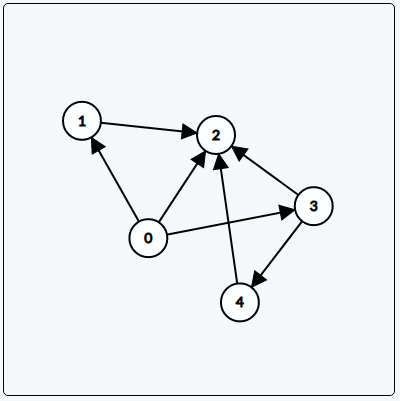
\includegraphics[scale= 0.6]{images/e2graph.png}
				\caption*{Ejercicio 2: Grafo a representar}
			\end{figure}
			
			\begin{figure}[H]
				\centering
				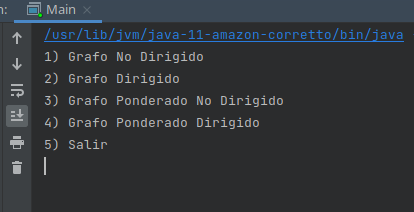
\includegraphics[scale= 0.9]{images/e21.png}
				\caption*{Ejercicio 2: Menu Principal}
			\end{figure}
			
			\begin{figure}[H]
				\centering
				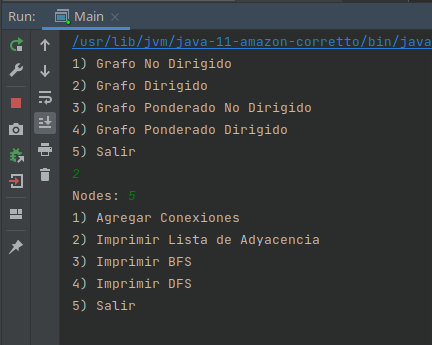
\includegraphics[scale= 0.9]{images/e22.png}
				\caption*{Ejercicio 2: submenu2, se agregan nodos}
			\end{figure}
			
			\begin{figure}[H]
				\centering
				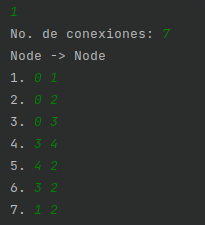
\includegraphics[scale= 1]{images/e23.png}
				\caption*{Ejercicio 2: Opcion 1, se agregan conexiones}
			\end{figure}
			
			\begin{figure}[H]
				\centering
				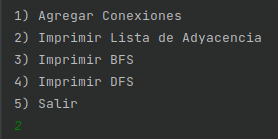
\includegraphics[scale= 1]{images/e24.png}
				\caption*{Ejercicio 2: Se imprime la lista de adyacencia}
			\end{figure}
			
			\begin{figure}[H]
				\centering
				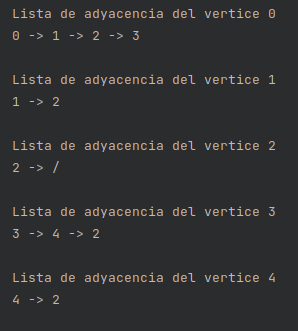
\includegraphics[scale= 1]{images/e25.png}
				\caption*{Ejercicio 1.2: Se visualiza la lista}
			\end{figure}
		
		\newpage
			
		\subsection{Ejercicio 3}
		
			\subsubsection{Desarrollo}
			
				Para este ejercicio una de las implementaciones que hice fue dentro de la clase \emph{Node} fue modficar su estrucutra a la siguiente:
				
				\begin{itemize}
					\item \textit{private LinkedList$<$Node$>$} \textbf{next}
					\item \textit{private LinkedList$<$Integer$>$} \textbf{edges}
					\item \textit{private int} \textbf{num}
					\item \textit{private int} \textbf{N}
					\item \textit{private int} \textbf{E}
				\end{itemize}
				
				La lista \textbf{next} contiene las \textbf{referencias} a otros nodos a los que hace adyacencia.\\
				
				La lista \textbf{edges} contiene el valor de los aristas a cada uno de esos nodos.\\
				
				La variable \textbf{num} contiene el numero que le corresponde a ese nodo.\\
				
				La variable \textbf{N} contiene la cantidad de nodos a los que hace adyacencia el nodo.\\
				
				La variable \textbf{E} contiene el mismo numero de nodos pero su distancia o costo en caso de que el grafo sea ponderado.\\
				
				Una de las cosas que hice, es que sobrecargue el metodo \emph{addNode()} dentro de la clase \emph{Node} para los grafos ponderados, de tal manera que al momento de crear un nodo, en vez de requerir unicamente el nodo a agregar dentro de la lista \textbf{next}, el metodo tambien requiere el valor del arista que se agrega junto con ese nodo y que inserta dentro de la lista \textbf{edges} al momento de ingresar el nodo.\\
				
				De igual manera para el metodo \emph{setEdges()} cuando se trata de grafos ponderados, en su segundo parametro utilizo la palabra \textbf{"p"} que se refiere a ponderado y al momento de hacer esto, el programa contiene instrucciones, para que en caso de que en el segundo parametro se encuentre esta palabra, entonces en vez de solicitar 2 variables que serian las de los grafos \textbf{v} y \textbf{w} tambien solicite la variable \textbf{e} que corresponde al valor de la arista.\\
				
				El programa tambien imprime antes de solicitar esta informacion la leyenda \textit{Node -$>$ Distancia -$>$ Node} que explica de que manera se debe de ingresar la informacion cuando se trata de un grafo ponderado, osea, debemos primero de ingresar la informacion del nodo a conectar, despues de la distancia o costo que se encuentra entre ambos nodos y al finalizar el nodo objetivo.\\
				
				Cuando el metodo \emph{setEdges()} identifica que el programa contiene una \textbf{"p"} como segundo argumento, entonces utiliza de igual forma, una de las versiones sobrecargadas de los metodos \emph(uGraphNodeAdd()) o \emph{dGraphNodeAdd()} las cuales contienen 3 parametros en vez de 2 que por su puesto, incluyen a la distancia entre los nodos.
				
				\newpage
				
			\subsubsection{Ejecucion}
			
			\textbf{Grafo Ponderado No Dirigido}\\
			
			\begin{figure}[H]
				\centering
				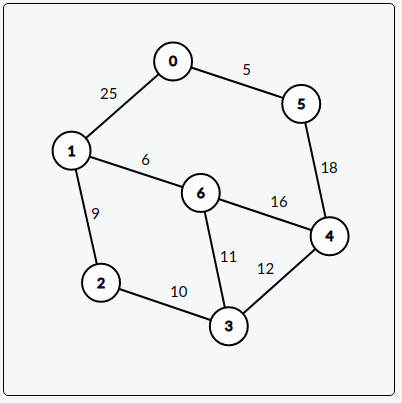
\includegraphics[scale= 0.6]{images/e3graph.png}
				\caption*{Ejercicio 3: Grafo a representar}
			\end{figure}
			
			\begin{figure}[H]
				\centering
				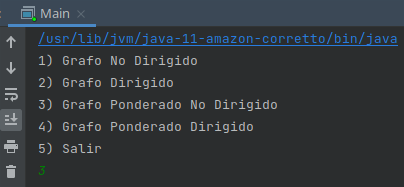
\includegraphics[scale= 0.9]{images/e31.png}
				\caption*{Ejercicio 2: Menu Principal}
			\end{figure}
			
			\begin{figure}[H]
				\centering
				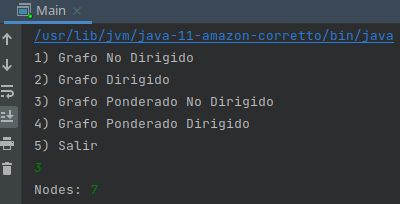
\includegraphics[scale= 0.9]{images/e32.png}
				\caption*{Ejercicio 3: submenu3, se agregan nodos}
			\end{figure}
			
			\begin{figure}[H]
				\centering
				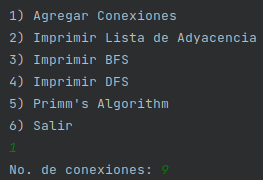
\includegraphics[scale= 1]{images/e33.png}
				\caption*{Ejercicio 3: Opcion 1, se agregan conexiones}
			\end{figure}
			
			\begin{figure}[H]
				\centering
				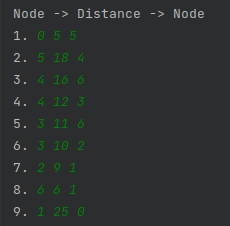
\includegraphics[scale= 1]{images/e34.png}
				\caption*{Ejercicio 3: Se incluyen los nodos y entre ambos la distancia}
			\end{figure}
			
			\begin{figure}[H]
				\centering
				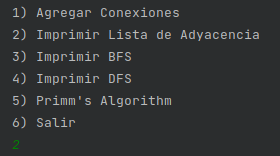
\includegraphics[scale= 1]{images/e35.png}
				\caption*{Ejercicio 3: Opcion 2 para visualizar lista de adyacencia}
			\end{figure}
		
			\begin{figure}[H]
				\centering
				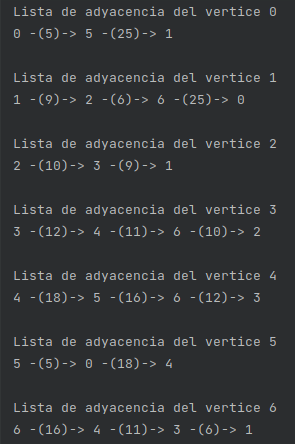
\includegraphics[scale= 1]{images/e36.png}
				\caption*{Ejercicio 3: Se visualiza la lista con distancia a cada Nodo}
			\end{figure}
		
			\newpage
		
			\textbf{Grafo Ponderado Dirigido}
			
			\begin{figure}[H]
				\centering
				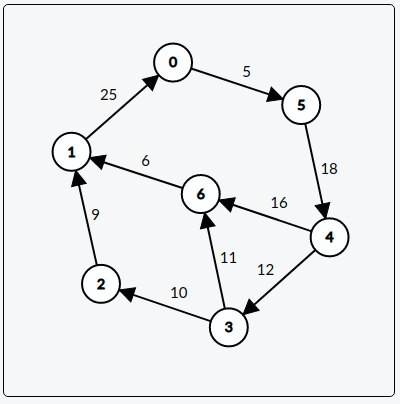
\includegraphics[scale= 0.8]{images/e3graph2.png}
				\caption*{Ejercicio 3: Grafo ponderado dirigido a representar}
			\end{figure}
			
			\begin{figure}[H]
				\centering
				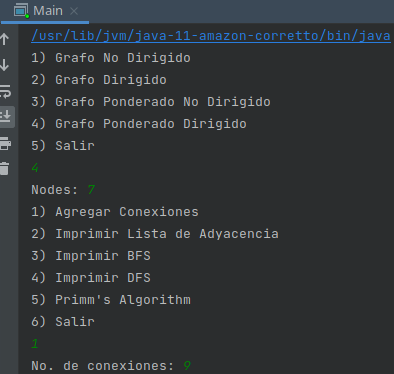
\includegraphics[scale= 0.9]{images/e37.png}
				\caption*{Ejercicio 2: Menu principal y se agregan nodos, menu3}
			\end{figure}
			
			\begin{figure}[H]
				\centering
				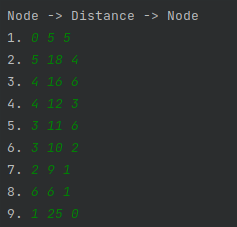
\includegraphics[scale= 0.9]{images/e38.png}
				\caption*{Ejercicio 3: Se agregan conexiones con distancia}
			\end{figure}
			
			\begin{figure}[H]
				\centering
				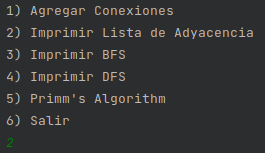
\includegraphics[scale= 1]{images/e39.png}
				\caption*{Ejercicio 3: Opcion 2 para imprimir lista de adyacencia}
			\end{figure}
			
			\begin{figure}[H]
				\centering
				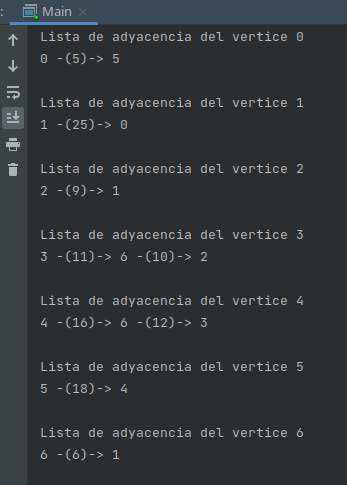
\includegraphics[scale= 1]{images/e310.png}
				\caption*{Ejercicio 3: Lista de adyacencia para grafo ponderado no dirigido}
			\end{figure}
			
		\newpage	
			
		\subsection{Ejercicio 4}
			
			\subsubsection{Desarrollo}
			
			Para el desarrollo de este ejercicio tuve que modificar el algoritmo mostrado en la practica para que fuera compatible con la estructura de datos que cree tanto para mi clase \emph{Nodo} como para mi clase \emph{Graph}.\\
			
			Una de las cosas que agregue, fue codigo en el metodo \emph{BFS()} para que este desde el interior del metodo, pregunte al usuario cual es el nodo por donde desea iniciar el recorrido del grafo por medio de un \textit{do-while loop} que verifica que el usuario ingrese un grafo existente para poder recorrerlo. De esta manera el metodo ya no usa ningun parametro y se vuelve mas dinamico.\\
			
			Despues, debido a la estructura de datos que implemente, removi el iterador porque tuve algunos problemas al momento de implementarlo y mejor lo sustitui por un \textit{enhanced for-loop} que itera dentro de la lista \verb|nodes.get(s).getNext()|, \textit{getNext()} es el \textit{"getter"} de la lista ligada de Nodos que el nodo contiene (sus conexiones) asi, ee codigo, devuelve una lista de nodos contenidos en el nodo con indice \textbf{s} de la lista de la clase \emph{Graph}.\\
			
			El funcionamiento de \emph{BFS()} me parecio muy sencillo, despues de escoger a partir de que nodo quieres comenzar a recorrer el la grafica. Se crea un arreglo de variables tipo \textit{boolean} del tamano de la cantidad de nodos contenidos en el grafo. Despues de esto se crea una lista ligada que contiene variables de tipo entero \textbf{queue} y se agrega dentro del indice \textbf{s} que previamente escogio el usuario, de el arreglo \textbf{visited} se iguala a \textit{true} indicando que ese nodo ya ha sido visitado.\\
			
			Por medio del metodo \emph{add()} se ingresa el valor numerico del nodo a la lista \textbf{queue} y se ingresa a un \textit{while-loop} que no termina sino hasta que el tamano de la lista \textbf{queue} sea igual 0.\\
			
			Dentro de este \textit{while-loop} se remueve el primer indice de \textbf{queue} por medio del metodo \emph{poll()} y se agrega este valor, nuevamente a la variable \textbf{s}. Despues de esto, como ya se habia comentado, se itera con un \textit{enhanced for-loop} a la lista de nodos contenidos dentro del nodo \textbf{s} y se obtiene el numero de cada nodo por medio del metodo \textit{getter} \verb|node.getNum()|, despues de esto se verifica si este nodo se encuentra dentro del arreglo \textbf{visited} en el indice que le corresponde, si no es asi, entonces se iguala ese indice a \textit{true} y se agrega a la \textbf{queue} por medio del metodo \emph{add()}. El ciclo termina de iterar cuando ya todos los espacios en visited son iguales a \textit{true} y consecuentemente no quedan nodos dentro de \textbf{queue}.
			
			\subsubsection{Ejecucion}
			
			\begin{figure}[H]
				\centering
				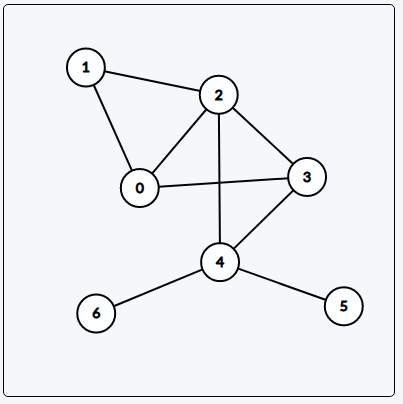
\includegraphics[scale= 0.6]{images/e4graph1.png}
				\caption*{Ejercicio 4: Grafo a representar}
			\end{figure}
			
			\begin{figure}[H]
				\centering
				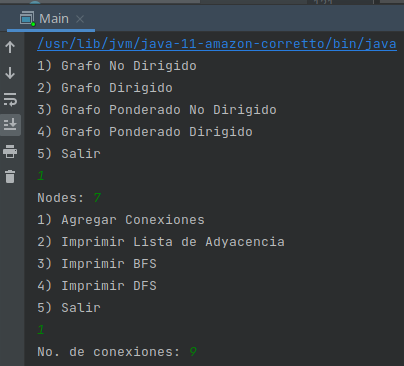
\includegraphics[scale= 0.75]{images/e41.png}
				\caption*{Ejercicio 4: Menu Principal agregamos nodos y conexiones}
			\end{figure}
			
			\begin{figure}[H]
				\centering
				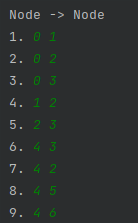
\includegraphics[scale= 0.9]{images/e42.png}
				\caption*{Ejercicio 4: Se agregan conexiones}
			\end{figure}
			
			\begin{figure}[H]
				\centering
				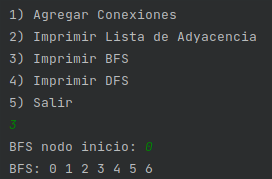
\includegraphics[scale= 1]{images/e43.png}
				\caption*{Ejercicio 4: BFS a partir de nodo 0}
			\end{figure}
			
			\begin{figure}[H]
				\centering
				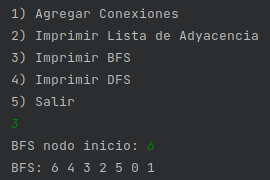
\includegraphics[scale= 1]{images/e44.png}
				\caption*{Ejercicio 4: BFS a partir de nodo 6}
			\end{figure}
			
			\begin{figure}[H]
				\centering
				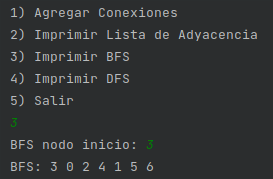
\includegraphics[scale= 1]{images/e45.png}
				\caption*{Ejercicio 4: BFS a partir de nodo 3}
			\end{figure}
			
			\begin{figure}[H]
				\centering
				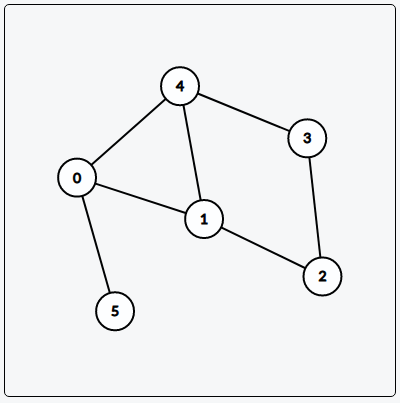
\includegraphics[scale = 0.7]{images/e4graph2.png}
				\caption*{Ejercicio 4: Grafo no 2}
			\end{figure}
		
			\begin{figure}[H]
				\centering
				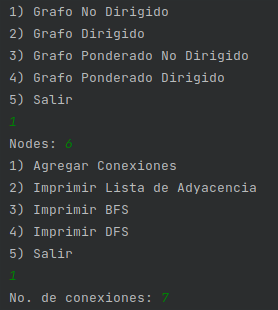
\includegraphics[scale= 0.9]{images/e46.png}
				\caption*{Ejercicio 4: Menu Principal y agregamos nodos y conexiones}
			\end{figure}
			
			\begin{figure}[H]
				\centering
				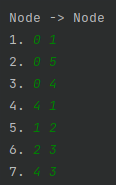
\includegraphics[scale= 0.9]{images/e47.png}
				\caption*{Ejercicio 4: Se asocian nodos}
			\end{figure}
			
			\begin{figure}[H]
				\centering
				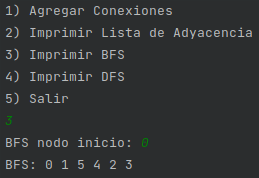
\includegraphics[scale= 1]{images/e48.png}
				\caption*{Ejercicio 4: BFS desde nodo 0}
			\end{figure}
			
			\begin{figure}[H]
				\centering
				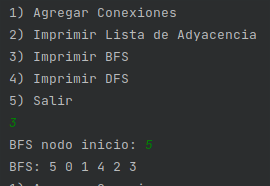
\includegraphics[scale= 1]{images/e49.png}
				\caption*{Ejercicio 4: BFS desde nodo 5}
			\end{figure}
			
			\begin{figure}[H]
				\centering
				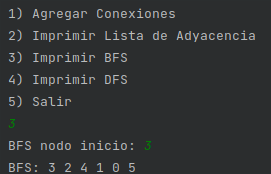
\includegraphics[scale= 1]{images/e410.png}
				\caption*{Ejercicio 4: BFS desde nodo 3}
			\end{figure}
		
		\newpage
			
		\subsection{Ejercicio 5}
			\subsubsection{Desarrollo}
			
			Para la implementacion de el metodo \emph{DFS()} las modificaciones que le tuve que hacer fueron similares a las de \emph(BFS()). De igual manera el usuario tiene la opcion de escoger el nodo a partir del cual quiere comenzar a recorrer el grafo de forma dinamica y dentro del cuerpo de \emph{DFSUtil()} tambien sustitui el iterador por un \textit{enhanced for-loop} que opera de la misma forma que en \emph{BFS()}.\\
			
			Algo que me llamo la antencion de \emph{BFS()} es que este opera de forma recursiva dentro del metodo \emph{DFSUtil()}.\\
			
			El metodo comienza con \emph{DFS()} que como ya lo mencionamos, pide al usuario el nodo por el cual quiere comenzar, de igual manera que \emph{DFS()} se crea un arreglo de \textit{boolean} llamado \textbf{visited} pero en este caso, tanto el nodo escogido por el usuario \textbf{v} como el arreglo \textbf{visited} se transfieren como parametros al metodo \emph{DFSUtil()}.\\
			
			Ya dentro de \emph{DFSUTil()} de igual forma se agrega dentro de \textbf{visited} en el indice \textbf{v} se iguala a \textit{true} y se comienza a iterar dentro del indice \textbf{v} de los nodos de la lista \textbf{nodes}, al igual que en el anterior, se declara una variable entera \textbf{n} que se iguala a \verb|node.getNum()| que proporciona el numero del nodo en cuestion. Si la variable \textbf{n} como nodo no esta contenida (no esta igualada a \textit{true}) dentro del indice \textbf{n} que le corresponde, entonces se invoca recursivamente a \emph{DFSUtil()} pero ahora con \textbf{n} como parametro para continuar el proceso de tal forma que se va iterando dentro de cada nodo como si fuera una linea hasta llegar a lo mas profundo de este a diferencia de \textbf{BFS()} que unicamente alcanza un nivel por debajo del nodo en cuestion para revisar sus contenidos.		
			
			\subsubsection{Ejecucion}
			
				\begin{figure}[H]
					\centering
					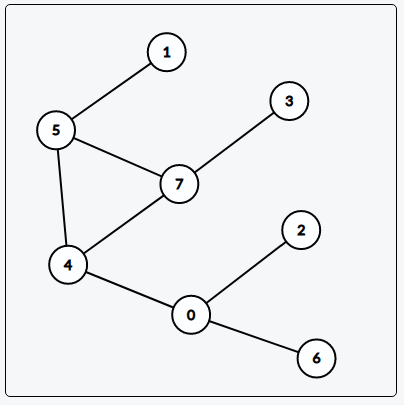
\includegraphics[scale= 0.6]{images/e5graph.png}
					\caption*{Ejercicio 5: Grafo a ingresar}
				\end{figure}
				
				\begin{figure}[H]
					\centering
					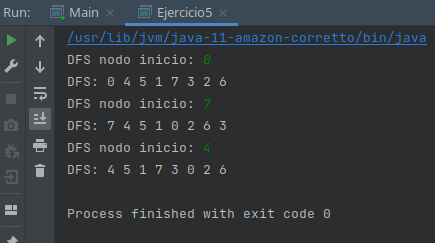
\includegraphics[scale= 0.7]{images/e51.png}
					\caption*{Ejercicio 5: Ejecucion DFS desde 3 nodos}
				\end{figure}
			
		\subsection{Ejercicio 6: Adicional}
		
			\subsubsection{Desarrollo}
				
				Aunque intente hacerlo por mi cuenta y sin verificar informacion de internet, no pude completar el algoritmo de Primm, pero seguire trabajando en el ya que dudo que haya estado lejos de comenzar a conseguir algo con el.\\
				
				El codigo se encuentra como metodo de la clase \emph{Graph}, el metodo se llama \emph{primm()} y se encuentra en la linea 176 de la clase.
				
			\newpage
	
	
	\section{Conclusiones}
	
		Esta practica me gusto mucho porque me puso a pensar muchisimo sobre los grafos y como se itera sobre ellos.\\
		
		Ya tenia yo una vaga idea sobre como debia de implementar los grafos en codigo debido a que alguna vez me puse a pensar en ello y decidi llevar manos a la obra durante la practica y ponerme a experimentar muchisimo ya que algo que me agrada es poder construir estructuras de datos a partir de nada y sin ayuda de muchos metodos predefinidos.
		
		Fue por esta razon que durante la practica me di a la tarea de implementar la idea que yo tenia de los elementos que un Nodo tenia que contener y por esta razon le implemente una lista ligada de otros nodos a los cuales pudiera tener referencia.\\
		
		Algo en lo que tambien me base fue en la definicion de grafos la cual menciona que es un conjunto $S = \{G, E\}$ donde \textbf{G} es el conjunto de grafos y \textbf{E} el conjunto de aristas. Fue en esto que me base para la clase \emph{Graph} que es precisamente lo que ahi representa \textbf{S} como el conjunto donde todos los grafos pertenecientes a un conjunto habitan.\\
		
		Lo que si me di cuenta de la practica es que ya no voy a estar experimentando tanto, porque hice bastantes metodos porque me gusta mi codigo genial, estructurado y eficiente. Pero me tardo mucho en hacerlo y luego ya no me da tiempo de acabar la practica por escrito y ando a las prisas. Una lastima porque me gusta mucho programar y experimentar con mi codigo.\\
		
		Espero que le guste mi practica y gracias por leerme\\
	
	
\end{document}